documentclass[tikz,border=5mm]{standalone}
\usetikzlibrary{shapes,arrows.meta,positioning}

\tikzset{
    % Define style for data points
    data/.style={
        rectangle,
        minimum width=2cm,
        text centered,
        draw,
        fill=red!40,
        rounded corners=0.5ex,
    },
    % Define style for data labels
    data_label/.style={
        rectangle,
        minimum width=2cm,
        text centered,
        draw,
        rounded corners=0.5ex,
        align=center
    },
    % Define style for publications
    publication/.style={
        rectangle,
        minimum width=2cm,
        text centered,
        draw,
        fill=green!40,
        rounded corners=0.5ex,
    },
    % Define style for collaborations
    collaboration/.style={
        rectangle,
        minimum width=2cm,
        text centered,
        draw,
        fill=cyan!40,
        rounded corners=0.5ex,
    },
    % Define style for institutions
    institution/.style={
        rectangle,
        minimum width=2cm,
        text centered,
        draw,
        fill=brown!40,
        rounded corners=0.5ex,
    },
    % Define style for other publications
    other_publication/.style={
        rectangle,
        minimum width=2cm,
        text centered,
        draw,
        fill=purple!40,
        rounded corners=0.5ex,
    },
    % Define style for arrows
    arrow/.style={-Stealth,line width=1pt},
    % Define style for timeline
    timeline/.style={
        -Stealth,line width=1pt,
    }
}

\begin{document}
    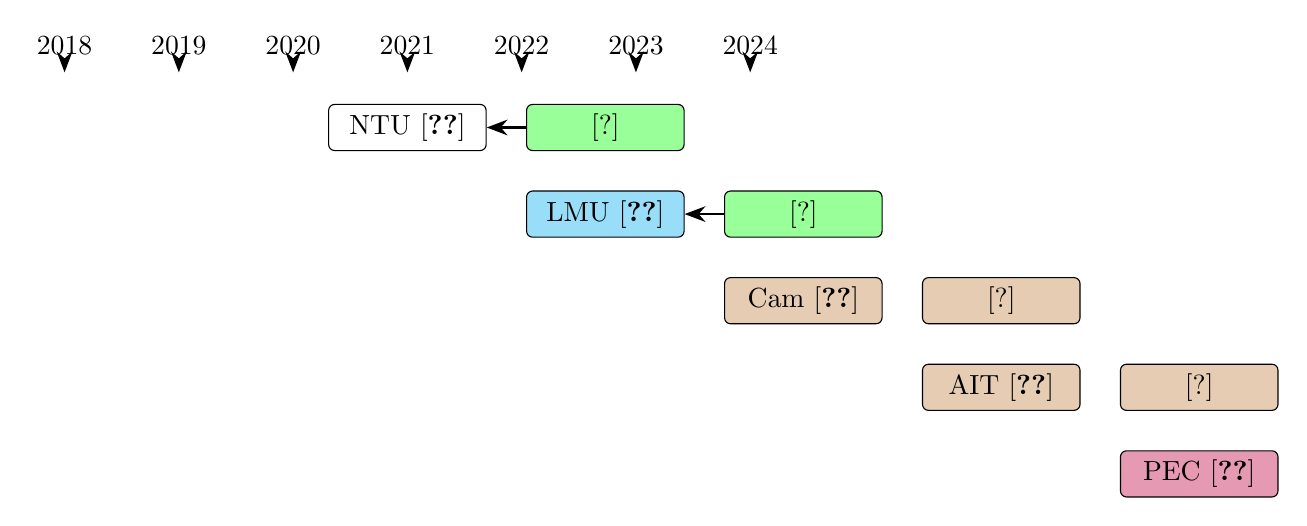
\begin{tikzpicture}[node distance=0.5cm]
        % Define nodes for timeline years
        \node (year_1) {2018};
        \node[right=of year_1] (year_2) {2019};
        \node[right=of year_2] (year_3) {2020};
        \node[right=of year_3] (year_4) {2021};
        \node[right=of year_4] (year_5) {2022};
        \node[right=of year_5] (year_6) {2023};
        \node[right=of year_6] (year_7) {2024};

        % Draw timeline
        \draw[timeline] (year_1.south) -- ++(0,-1mm);
        \draw[timeline] (year_2.south) -- ++(0,-1mm);
        \draw[timeline] (year_3.south) -- ++(0,-1mm);
        \draw[timeline] (year_4.south) -- ++(0,-1mm);
        \draw[timeline] (year_5.south) -- ++(0,-1mm);
        \draw[timeline] (year_6.south) -- ++(0,-1mm);
        \draw[timeline] (year_7.south) -- ++(0,-1mm);

        % Draw nodes for publications
        \node[data_label,below=of year_4] (ntu) {NTU [\ref{ntu}]};
        \node[publication,right=of ntu] (ntu_pub) {[?]};

        % Draw nodes for collaborations
        \node[collaboration,below=of ntu_pub] (lmu) {LMU [\ref{lmu}]};
        \node[publication,right=of lmu] (lmu_pub) {[?]};

        % Draw nodes for institutions
        \node[institution,below=of lmu_pub] (cam) {Cam [\ref{cam}]};
        \node[institution,right=of cam] (cam_collab) {[?]};

        % Draw nodes for other publications
        \node[institution,below=of cam_collab] (ait) {AIT [\ref{ait}]};
        \node[institution,right=of ait] (ait_collab) {[?]};

        % Draw nodes for other publications
        \node[other_publication,below=of ait_collab] (pec) {PEC [\ref{pec}]};

        % Draw arrows between nodes
        \draw[arrow] (ntu_pub.west) -- (ntu.east);
        \draw[arrow] (lmu_pub.west) -- (lmu.east);
    \end{tikzpicture}
\end{document}